\paragraph{1. Dependancy toevoegen}
Om de NotificationCompat API te kunnen gebruiken, moeten er normaal gezien geen extra dependancies worden toegevoegd.
Maar er moet wel gecontroleerd worden of de volgende dependancy aanwezig is.
\begin{minted}{java}
  val core_version = "1.6.0"
  dependencies {
      implementation("androidx.core:core-ktx:$core_version")
  }
\end{minted}

\paragraph{2. Notificatie aanmaken}
Om een notificatie aan te maken, moet de NotificationCompat.Builder object worden gebruikt. 
\begin{minted}{kotlin}
  private fun createNotification(title: String, body: String) {
    val builder = NotificationCompat.Builder(this, CHANNEL_ID)
      .setSmallIcon(icon)
      .setContentTitle(title)
      .setContentText(body)
      .setPriority(NotificationCompat.PRIORITY_DEFAULT)

    val notificationManager: NotificationManager =
      getSystemService(Context.NOTIFICATION_SERVICE) as NotificationManager
    notificationManager.notify(notificationId, builder.build())
}
\end{minted}
\begin{figure}[H]
    \centering
    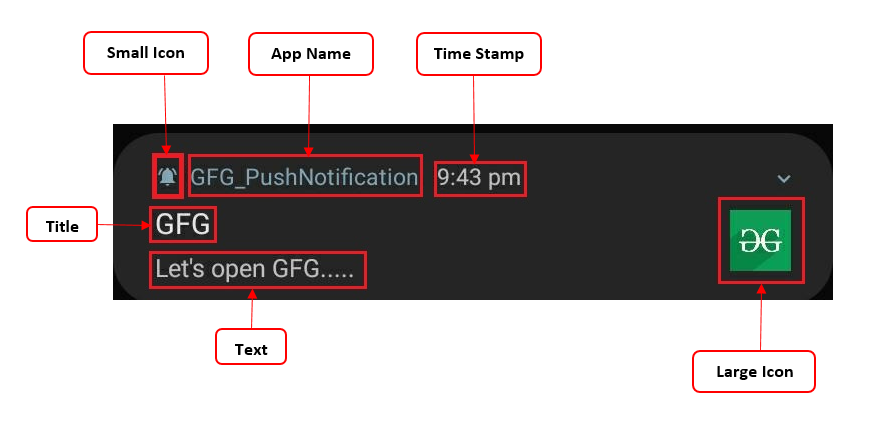
\includegraphics[height=0.3\textheight]{NotificationAnatomy.png}
    \caption{Anatomy standaard notificatie \parencite{One2020}.}
\end{figure}

\paragraph{3. Channel aanmaken}
Het laatste dat nodig is vooraleer de notificatie getoond kan worden, is een channel. Deze wordt 
gebruikt om notificaties te groeperen volgens hun belang. Om een channel aan te maken, wordt  
de .createNotificationChannel() methode gebruikt. Het maakt niet uit wanneer of waar deze wordt uitgevoerd. 
Het is enkel belangrijk dat de channel wordt aangemaakt vooraleer notificaties 
worden getoond. Dus best zo vroeg mogelijk in de applicatie.
\begin{minted}{kotlin}
private fun createNotificationChannel() {
  if (Build.VERSION.SDK_INT >= Build.VERSION_CODES.O) {
    val name = "bachproef"
    val descriptionText = "bachproef notificaties"
    val importance = NotificationManager.IMPORTANCE_DEFAULT
    val channel = NotificationChannel(CHANNEL_ID, name, importance).apply {
      description = descriptionText
    }
    // Channel bij het systeem registreren
    val notificationManager: NotificationManager =
      getSystemService(Context.NOTIFICATION_SERVICE) as NotificationManager
    notificationManager.createNotificationChannel(channel)
  }
}
\end{minted}

\paragraph{4. Applicatie maken}
Met deze informatie kan er een applicatie worden opgebouwd die notificaties zal sturen. De applicatie bestaat 
uit twee \textbf{EditText} componenten voor de titel en beschijving van de notificatie en tot slot een 
\textbf{Button} om de notificatie te triggeren. Als de knop wordt ingedrukt dan wordt de 
\textbf{createNotification} methode aangeroepen en wordt de waarde van de inputs meegegeven.
\begin{figure}[H]
  \centering
  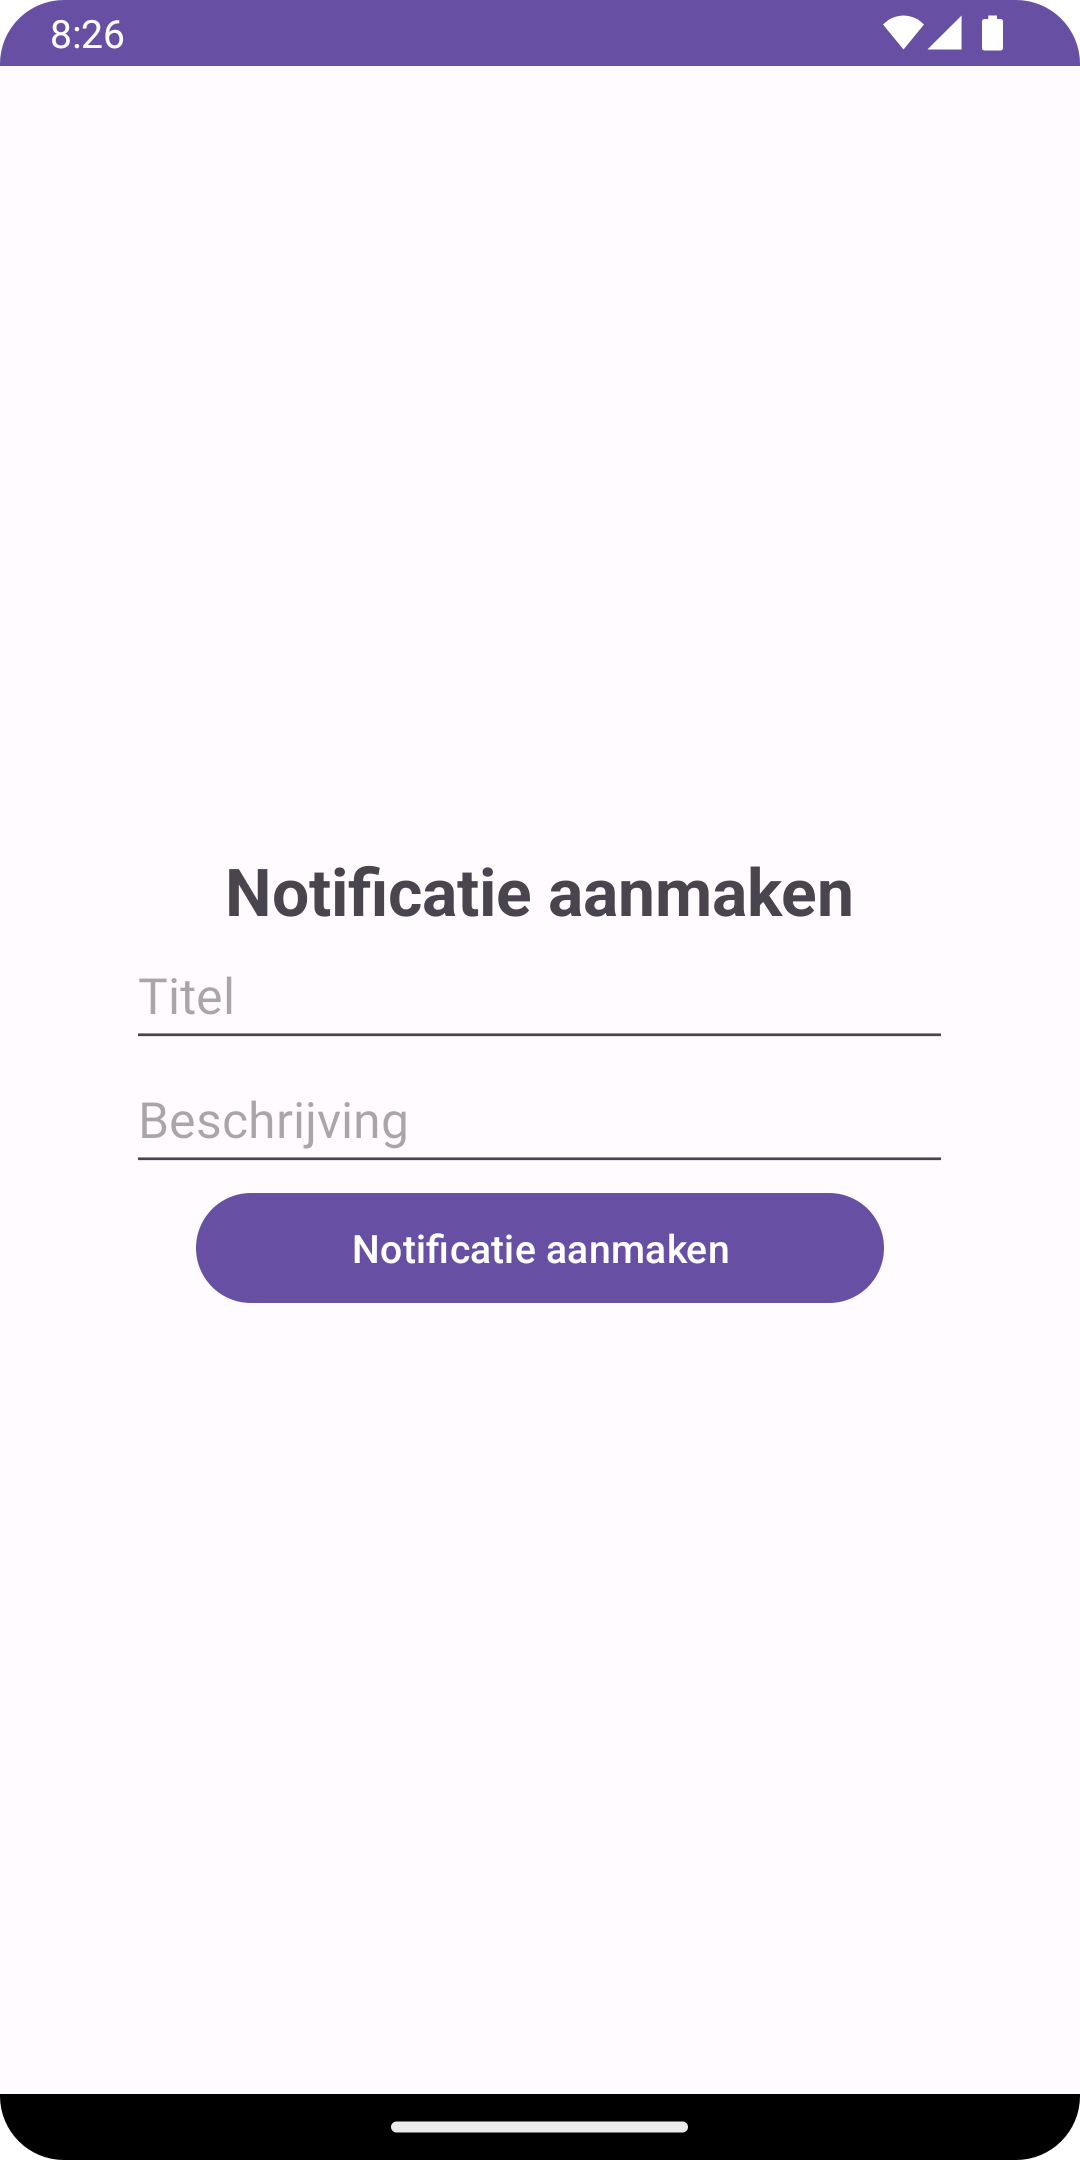
\includegraphics[height=0.4\textheight]{notificaties_layoutnative.png}
  \caption{Layout van applicatie voor notificaties te sturen bij Android.}
\end{figure}